\chapter{Structure of the verb}
\section{Introduction}
The purpose of this chapter is to give an introduction to the phonological and morphological structure of the verbal word in Nyakyusa, as well as to give a description of several morphemes that do not fit in the following chapters.

First, the phonological structure of verbal morphemes will be laid out (\sectref{PhonologicalStructureVerbalMorphemes}), followed by a description of the linear morphological structure of the finite verb (\sectref{LinearStructureOFiniteVerb}). The latter includes a description of each of the slots that make up the finite verbs and the morphemes that may fill these slots. Specific focus is laid on subject\is{subject marker} and object prefixes\is{object marker} as well as on post-final enclitics.\is{enclitic} Last, the hierarchical structure of the verbal root,\is{root} \isi{base} and \isi{stem} will be discussed (\sectref{RootBaseStem}).

\section{Phonological structure of verbal morphemes}\label{PhonologicalStructureVerbalMorphemes}
The basic segmental shape of the verbal \isi{root} is CVC, where C\textsubscript{1} can be followed by a glide and C\textsubscript{2} can be a prenasalized plosive; C\textsubscript{1} is never prenasalized. One of the consonantal segments can be zero and V might be short or long. For vowel-initial roots,\is{root} all vowels in the inventory but /u/ are attested, which is most likely an accidental gap, as nominal stems with initial /u/ are attested, e.g. \textit{ʊ}-\textit{mu}-\textit{unyu} `salt', \textit{ɪ}-\textit{ly}-\textit{ungu} `pumpkin'.

Although disyllabic roots\is{root} can be considered the most basic structure, more complex forms outnumber these in the present-day language. Most verbs with a more complex shape can be analysed as the outcome of derivational\is{derivation} processes, although in many cases such an analysis can only be arrived at through a comparative Bantu perspective. Only 17 monosyllabic verbs exist in Nyakyusa. These, however, include some very basic concepts. (\ref{exMonosyllabycStems}) lists their isi{stem} forms; see \sectref{RootBaseStem} on roots\is{root} and stems.\is{stem} Note that <ni> in \textit{nia} stands for a sequence of coronal nasal plus palatal glide.

\clearpage

\begin{exe}
	\ex\label{exMonosyllabycStems}
	\begin{multicols}{2}
		\begin{xlist}
			\ex
			\begin{tabbing}
				mwx\=\kill
				shape Cɪ (defective verbs) \\
				\textit{lɪ}\>`be'\\
				\textit{tɪ}\>`say; think; do like'
			\end{tabbing}
			\ex shape C(V)-a
			\begin{tabbing}
				\textit{pa} (p(a)-a)x\=\kill
				\textit{pa} (p(a)-a)\>`give'\footnotemark\\
				\textit{ja} (j-a)\>`be, become'
			\end{tabbing}
			\footnotetext{The verb \textit{pa} \lq give' behaves ambiguously with regard to its segmentation. Both vowel quality and length\is{vowels!length} in the perfective stem \textit{peele} (\sectref{Imbrication}), the \isi{applicative} \textit{peela} (\sectref{MorphophonologyOfVerbalExtension}) and the passive\is{passive!productive} \textit{peegwa} (\sectref{Passive}) indicate a root \textit{pa}. With the imperfective suffix however, the stem takes the shape \textit{paga} (\textit{pege} in the imperfective subjunctive), not \textit{*paaga, peege}. With post-final clitics\is{enclitic} it also surfaces as \textit{pa} (\textit{pe} in the subjunctive). Thus it is treated as \textit{p} in these cases.}
			\ex shape Cy-a
			\begin{tabbing}
				mwax\=\kill
				\textit{kya}	\>`cease raining; dawn'\\
				\textit{lya}	\>`eat'\\
				\textit{nia}	\>`defecate'\\
				\textit{pya}	\>`be burnt'\\
				\textit{sya}	\>`grind'
			\end{tabbing}
			\columnbreak
			\ex shape Cw-a
			\begin{tabbing}
				mwax\=\kill
				\textit{fwa}\>`die'\\
				\textit{gwa}	\>`fall'\\
				\textit{kwa}	\>`pay dowry'\\
				\textit{lwa}	\>`fight'\\
				\textit{mwa}	\>`shave'\\
				\textit{nwa}	\>`drink'\\
				\textit{swa}	\>`spit; forgive'\\
				\textit{twa}	\>`be plenty (esp. of fish)'
			\end{tabbing}
		\end{xlist}
	\end{multicols}
\end{exe}

\noindent The typical verbal prefix has the shape CV-, with a very limited number of exceptions having VCV-, V- or N-. Prefixes do not contain the mid vowels /e/ and /o/. Suffixes typically have the mirrored form -VC, with a few cases of -V. Of the few suffixes having -VCV, some might be understood as bipartite -VC-V. The final vowel segment of the verbal word is always short. This also holds when post-final clitics (\sectref{PostfinalClitics})\is{enclitic} are attached.
\section{Linear morphological structure of the finite verb}\label{LinearStructureOFiniteVerb}
The highly agglutinative structure of the finite verb in Nyakyusa can be understood as consisting of a number of slots for derivational and inflectional affixes that frame the basic unit, the verbal root.\is{root}

The linear arrangement of the verbal morphemes and the functions associated with each slot can be represented as in \figref{Linearstructureofthefiniteverb}, adopting the segmentation and terminology proposed by \citet[546]{GueldemannT1999}. Slots with a subscript N may be filled with various affixes, as will be described in the corresponding sections.


\begin{figure}[H] % [H] sorgt dafür, dass genau hier und nicht verrutscht
	\label{FigLinearStructureOFiniteVerb}
	\centering
	\begin{tabular}{rccccc}
		\footnotesize{slot} & pre-initial & initial & post-initial\textsubscript{N} & pre-radical & radical\\
		\footnotesize{function} & tense/ & subject & TMA/ & object & verbal \\
		& emphasis & & polarity & & root\\[7.5pt]
		\footnotesize{slot} & pre-final\textsubscript{N} & final & post-final& \\
		\footnotesize{function} & derivation/ & TMA & locative/WH/ \\
		&  voice & & adverbial &
	\end{tabular}
	\caption{Linear structure of the finite verb}
	\label{Linearstructureofthefiniteverb}
\end{figure}

Examples (\ref{exImperativeAsMinimalVerb}) and (\ref{exMaximalVerb}) illustrate the imperative as the morphologically minimal possible structure and the use of all verbal slots respectively.\footnotemark

\begin{exe}
	\ex \label{exImperativeAsMinimalVerb}
	\gll job-a\\
	speak-\textsc{fv}\\
	\glt `Speak!'
	
	\ex
	\label{exMaximalVerb}
	\gll aa=tʊ-ti-kʊ-ba-jaat-ɪl-a=ko\\
	\textsc{fut}=\textsc{1pl}-\textsc{neg}-\textsc{prs}-2-walk-\textsc{appl}-\textsc{fv}=17(\textsc{loc})\\
	\glt `We will not visit them there'
\end{exe}
\footnotetext{The gloss \textsc{prs} `present' is here to be understood as shorthand for a non-past imperfective;\is{aspect!imperfective} see \sectref{Present}.}

In the following subsections, each of the individual slots, together with the morphemes that may fill them, will be described.

\subsection{The pre-initial slot}
The pre-initial slot of the verbal word may only contain a single morpheme. As \citet[186]{GueldemannT2003} notes, morphemes in this slot are typically the result of the truncation of a formerly bi-predicate structure. This is most likely the case for the de-itive future proclitic\is{proclitic} \textit{aa}= (\sectref{ProcliticAa}) and its de-ventive counterpart (\textit{i})\textit{sa}= (\sectref{ProcliticIsa}). Other morphemes that may occupy this slot are a proclitic\is{proclitic} form of comitative \textit{na}= as well as a proclitic\is{proclitic} \textit{a}=, both of which add specific interlocutory and modal nuances to certain uses of the subjunctive paradigm (\sectref{SubjunctiveMainClause}). Last, in some southern varieties of Nyakyusa,\is{dialects} a proclitic\is{proclitic} \textit{naa} with a future-oriented meaning is found (\sectref{ProcliticNaa}), which might be a portmanteau of comitative \textit{na} and the future proclitic\is{proclitic} \textit{aa}=.

\subsection{The initial slot}
\label{SubjectConcords}
In the initial slot of the verbal word, the subject is marked.\is{subject marker} Any finite Nyakyusa verb, with the exception of imperatives (\sectref{Imperative}) and subjunctives in their directive use (\sectref{SubjunctiveMainClause}), carries a subject prefix. 

In the Bantuist and general linguistic tradition, the subject prefixes,\is{subject marker} as well as the object prefixes\is{object marker} (\sectref{ObjectConcords}), are most often referred to as \textit{agreement} markers. Given the origin of the term agreement in the treatment of person-marking in European languages and the typological problems associated with it (see e.g. \citealt{HaspelmathM2013}), the more neutral and also widespread term \textit{cross-reference} is used throughout this study. This nomenclature has the further advantage of capturing not only subject-\is{subject marker} and object-markers\is{object marker} but also the \isi{locative} morphemes described in \sectref{LocativeEnclitics}.

\is{subject marker|(}Concerning the subject markers, two paradigmatic sets of prefixes will be assumed in this study. The choice between the sets depends on the following formant: when the subject prefix directly precedes the simple present prefix \textit{kʊ}-, set 2 is used. Otherwise set 1 is used.

These two distinct sets are postulated for two reasons. First, the subject prefix for the second person singular is zero before \isi{simple present} \textit{kʊ}- and has the shape (\textit{g})\textit{ʊ}- elsewhere. Second, the shape of the other subject prefixes preceding \textit{kʊ}- is not completely predictable in the varieties that are in the focus of this study. While /a/ regularly changes to /i/ in this environment and the front vowel of some subject prefixes is raised to /i/, this is not a regularly predictable process (see Tables \ref{tableSMparticipants} and \ref{tableSMNCL}). In other topolects,\is{dialects} such as the one described by \citet{BergerP1938} and the lake-shore-plains variety,\is{dialects} which is the subject of ongoing research by SIL International, there is greater regularity. In those varieties all unrounded vowels preceding \isi{simple present} \textit{kʊ}- are raised to /i/ and all rounded back vowels change to /u/. The findings of the present study, however, basically agree with those of \citet{MwangokaNVoorhoeveJ1960b} and \citet{LabroussiC1998}. While the former work gives no information as to the variety studied, Labroussi's main assistant is a speaker of the Kukwe/Ngumba topolect.\is{dialects}

Similar alternations, in which a vowel segment /i/ surfaces in at least one allomorph of the \isi{simple present} (and constructions based on this paradigm), are found in numerous languages in a coherent area encompassing Nyakyusa as well as most of Guthrie's zones G60 and N10.\footnote{The variety of \ili{Ngonde} described by \citet{KishindoP1999} does not have this alternation in subject prefixes. This seemingly also holds for the \ili{Ngonde} described by \citet{LabroussiC1998}.} \citet{PersohnBBernanderR2016} trace this back to a \isi{grammaticalization} process the source structure of which consists of a reflex of \ili{Proto-Bantu} *\textit{jìkad} \lq dwell, be, sit' plus infinitive and the cradle of which is found in zone G60. 

In the following subsections, first the subject prefixes for the \isi{discourse participants} (first and second person) will be described (\sectref{SubjectConcordsParticipants}), followed by the prefixes for the \isi{noun classes} (third persons) (\sectref{SubjectConcordsNCL}). 
\subsubsection{Participant subject prefixes}
\label{SubjectConcordsParticipants}
\is{discourse participants|(}The subject prefixes for the discourse participants are listed in \tabref{tableSMparticipants}.\footnote{The second person plural is also used as an honorific. This usage seems to be limited to the exchange of greetings; also see \citet[32]{WalshM1982}.}

\begin{table}[H]%[HBT]
	\begin{center}
		\begin{tabular}{ccc}
			\lsptoprule 
			\footnotesize{Participant} & \footnotesize{Set 1} & \footnotesize{Set 2}\\ 
			\midrule 
			1\textsc{sg} & \textit{n}- & \textit{n} (\textit{ni}-) \\ 
			2\textsc{sg} & \textit{ʊ}- & \textit{ø}-\\ 
			1\textsc{pl} & \textit{tʊ}- & \textit{tʊ}-\\ 
			2\textsc{pl} & \textit{mu}- & \textit{mu}-\\
			\lspbottomrule 
		\end{tabular}
		\caption{Participant subject prefixes}
		\label{tableSMparticipants}
	\end{center}
\end{table}

The prefixes of the first and second person singular display some morphophonemic peculiarities. In the first person singular, set 2 contains an alternative form \textit{ni}-. This was found in older descriptions and text collections (e.g. \citealt{SchumannK1899}; \citealt{EndemannC1914}; \citealt{BergerP1933}). The younger speakers consulted were unaware of this alternation and it was considered antiquated by the older generation.

Preceding those noun class object prefixes\is{object marker} featuring a voiceless plosive (noun classes 7, 12, 13, 15, 16 and 17), the first person singular subject prefix is realized as a syllabic nasal. This is illustrated in (\ref{exSM1SGsyllabischvorOMNCL}). Before any other prefix with an initial voiceless plosive, it regularly triggers prenasalisation; see (\ref{exSM1SGsnichyllabischvorOMparticipants}) for the object prefixes of the second person singular and first person plural, and (\ref{exSM1SGsnichyllabischvorTMA}) for TMA prefixes. For stem-initial plosives see (\ref{exNC1sg}) in \sectref{PrenasalizedPlosives}. This allopmorphy can hence not be accounted for on a purely phonological base.

\begin{exe}
	\ex\label{exSM1SGsnichyllabischvorOMparticipants}
	\begin{tabbing}
		\textit{mpameenye}x\=(\degree n-pa-many-ile)x\=\kill
		\textit{ngʊmeenye}\>(\degree n-kʊ-many-ile)\>`I know you'\\
		\textit{ndʊmeenye}\>(\degree n-tʊ-many-ile)\>`I know us'
	\end{tabbing}

\clearpage

	\ex\label{exSM1SGsnichyllabischvorTMA}
	\begin{tabbing}
		\textit{mpameenye}x\=(\degree n-pa-many-ile)x\=\kill
		\textit{ngamanya}\>(\degree n-ka-many-a)\>`I do not know'\\
		\textit{ngamanye}\>(\degree n-ka-many-e)\>`I should go get to know'\\
		\textit{ndikʊjoba}\>(\degree n-ti-kʊ-job-a)\>`I do not speak'
	\end{tabbing}
	\ex \label{exSM1SGsyllabischvorOMNCL}
	\begin{tabbing}
		\textit{mpameenye}x\=(\degree n-pa-many-ile)x\=\kill
		\textit{nkameenye}\>(\degree n-ka-many-ile)\>`I know it (class 12)'
		\\\textit{ntʊmeenye}\>(\degree n-tʊ-many-ile)\>`I know them (class 13)'
		\\\textit{nkʊmeenye}\>(\degree n-kʊ-many-ile)\>`I know it (class 15)'
		\\\textit{mpameenye}\>(\degree n-pa-many-ile)\>`I know the place (class 16)'
		\\\textit{nkʊmeenye}\>(\degree n-kʊ-many-ile)\>`I know the place (class 17)'
	\end{tabbing}
\end{exe}

\label{MorphophonSM1SG} The first person singular subject prefix also surfaces as a syllabic nasal before a fricative or another nasal:
\begin{exe}
	\ex
	\begin{tabbing}
		\textit{mmumeenye}x\=(\degree n-mu-many-ile)x\=\kill
		\textit{mmalile}\>(\degree n-mal-ile)\>`I have finished' \\
		\textit{mmumeenye}\>(\degree n-mu-many-ile)\>`I know it inside (class 18)' \\
		\textit{nnusiisye}\>(\degree n-nus-ile)\>`I have smelled'\\
		\textit{nng'walile}\>(\degree n-ng'wal-ile)\>`I have scratched'\\
		\textit{nnyeelile}\>(\degree n-nyeel-ile)\>`I have jumped'\\
		\textit{nhobwike}\>(\degree n-hobok-ile)\>`I have rejoiced'\\
		\textit{mfibwene}\>(\degree n-fi-bon-ile)\>`I have seen them (class 8)' \\
		\textit{mfumile}\>(\degree m-fum-ile)\>`I have come (from)' \\
		\textit{nsibwene}\>(\degree n-si-bon-ile)\>`I have seen them (class 10)' \\
		\textit{nswile}\>(\degree n-sw-ile)\>`I have spilled' 
	\end{tabbing}
\end{exe}

\label{MonosyllabicSubjunctives}The first person singular subject prefix is further realized as a syllabic nasal before monosyllabic stems with an initial plosive or approximant in the subjunctive mood,\is{mood!subjunctive} that is, in those cases in which prenasalization would result in a monosyllabic word (\ref{exSM1SGMonosyllabicSubjunctive}). In the imperfective subjunctive\is{mood!subjunctive} and when post-final clitics\is{enclitic} are attached, the resultant word is no longer monosyllabic and the prefix surfaces as prenasalization (\ref{exSM1SGMonosyllabicSubjunctiveLongerWord}). Likewise, when the subjunctive of \textit{tɪ} \lq say; think; do like' merges with the following interrogative \textit{bʊle} (see \sectref{SubjunctiveTiBule}), the first person singular subject prefix surfaces as prenasalization (\ref{exSM1SGMonosyllabicSubjunctiveBule}). A similar avoidance of monosyllabic words is found with the corresponding object prefix in the imperative;\is{mood!imperative} see \sectref{sectionParticipantOM}.

\begin{exe}
	\ex \label{exSM1SGMonosyllabicSubjunctive}
	\begin{tabbing}
		\textit{ndʊbʊle}x\=(\degree n-lw-e=po)x\=\kill %unsinnszeile für tabulatoren
		\textit{n̩je} \> (\degree n-j-e) \> \lq I should be(come)'\\
		\textit{n̩dye} \> (\degree n-ly-e) \> \lq I should eat'\\
		\textit{n̩dɪ} \> (\degree n-tɪ) \> \lq I should say'\footnotemark\\
		\textit{n̩gwe} \> (\degree n-gw-e) \> \lq I should fall' % %muessen ja nicht ALLE gelistet werden
	\end{tabbing}
	\ex \label{exSM1SGMonosyllabicSubjunctiveLongerWord}
	\begin{tabbing}
		\textit{ndʊbʊle}x\=(\degree n-lw-e=po)x\=\kill %unsinnszeile für tabulatoren
		%\textit{ndwege} \> (\degree n-lw-ege) \> \lq I should be fighting'\\
		\textit{ndyege} \> (\degree n-ly-ege) \> \lq I should be eating'\\
		\textit{ndyepo} \> (\degree n-ly-e=po) \> \lq I should eat a bit'\\
		\textit{ndyemo} \> (\degree n-ly-e=mo) \> \lq I should eat some'\\
		\textit{ndɪgɪ} \> (\degree n-t-ɪgɪ) \> \lq I should be saying'
	\end{tabbing}
	\ex \label{exSM1SGMonosyllabicSubjunctiveBule}
	\begin{tabbing}
		\textit{ndʊbʊle}x\=(\degree n-lw-e=po)x\=\kill %unsinnszeile für tabulatoren
		\textit{ndʊbʊle} \> (\degree n-tɪ bʊle) \> \lq What should I say/do'
	\end{tabbing}
\end{exe}
\protect\footnotetext{For the subjunctive of defective \textit{tɪ}, see \sectref{defectiveti}.}

When the object prefix of noun class 1\is{object marker} follows the subject prefix of \textsc{1sg}, an epenthetic vowel /u/ is inserted.
\begin{exe}
	\ex \label{exSM1SGvorOM1}
	\begin{tabbing}
		\textit{nummʊʊliile}x\=(\degree n-mu-ʊl-ɪl-ile)x\=`I have bought for him \=\kill
		\textit{nummʊʊliile}\>(\degree n-mu-ʊl-ɪl-ile)\>`I have bought for him/her'\\
		\textit{nummwagile}\>(\degree n-mu-ag-ile)\>`I have found him/her'\\
		\textit{nunkomile}\>(\degree n-mu-kom-ile)\>`I have hit him/her'
	\end{tabbing}
\end{exe}

A vowel following the first person singular subject prefix is regularly long (\ref{exSM1SGFolgeVokalLang}),\is{vowels!length} with the exception of the indefinite future prefix \textit{isakʊ}- (\sectref{isaFut}).
\begin{exe}
	\ex \label{exSM1SGFolgeVokalLang}
	\begin{tabbing}
		\textit{naataagile}x\=(\degree n-a-taag-ile)x\=`I threw'\kill
		\textit{niisile}\>(\degree n-is-ile)\>`I have come'\\
		\textit{nɪɪmile}\>(\degree n-ɪm-ile)\>`I have stopped'\\
		\textit{neegile}\>(\degree n-eg-ile)\>`I have taken'\\
		\textit{naagile}\>(\degree n-ag-ile)\>`I have found'\\
		\textit{naataagile}\>(\degree n-a-taag-ile)\>`I threw'\\
		\textit{noogile}\>(\degree n-og-ile)\>`I have bathed'\\
		\textit{nʊʊlile}\>(\degree n-ʊl-ile)\>`I have bought'
	\end{tabbing}
\end{exe}

The subject prefix of the second person singular is realized as \textit{gʊ}- preceding a vowel (\ref{exSM2SGvorVokal}). The usual rules for vowel juxtaposition apply (see \sectref{HiatusSolution}).\is{vowels!hiatus solution}
\begin{exe}
	\ex \label{exSM2SGvorVokal}
	\begin{tabbing}
		\kill
		\textit{gwataagile}x\=(\degree ʊ-a-taag-ile)x\=`You threw'\kill
		\textit{gwisile}\>(\degree ʊ-is-ile)\>`you have come'\\
		\textit{gwɪmile}\>(\degree ʊ-ɪm-ile)\>`you have stopped'\\
		\textit{gwegile}\>(\degree ʊ-eg-ile)\>`you have taken'\\
		\textit{gwagile}\>(\degree ʊ-ag-ile)\>`you have found'\\
		\textit{gwataagile}\>(\degree ʊ-a-taag-ile)\>`you threw'\\
		\textit{googile}\>(\degree ʊ-og-ile)\>`you have bathed'\\
		\textit{gʊʊlile}\>(\degree ʊ-ʊl-ile)\>`you have bought'
	\end{tabbing}
\end{exe}

When the subject prefix of the second person singular is adjacent to the object prefix\is{object marker} of the first person singular or noun class 1, there is free variation between \textit{gʊ}- and \textit{ʊ}-. The only paradigms in which these two sets of morphemes can be adjacent are the subjunctive (\sectref{Subjunctive})\is{mood!subjunctive} and the present perfective (\sectref{PresentPerfective}):

\clearpage

\begin{exe}
	\ex \label{exSM2sgOM1SG}
	Subject prefix \textsc{2sg} and object prefix \textsc{1sg}:
	\begin{tabbing}
		\textit{(g)ʊʊnyʊʊliile}x\=(\degree ʊ-ny-ʊl-ɪl-ile)x\=`you have bought for me'\kill
		\textit{(g)ʊʊnyʊʊliile}\>(\degree ʊ-ny-ʊl-ɪl-ile)\>`you have bought for me'
		\\\textit{(g)ʊndaagile}\>(\degree ʊ-ny-taag-ile)\>`you have thrown me'
		\\\textit{(g)ʊʊsalile}\>(\degree ʊ-ny-sal-ile)\>`you have chosen me'
		\\\textit{(g)ʊʊnyʊʊlɪle}\>(\degree ʊ-ny-ʊl-ɪl-e)\>`you should buy for me'
		\\\textit{(g)ʊndaage}\>(\degree ʊ-ny-taag-e)\>`you should throw me'
		\\\textit{(g)ʊʊsale}\>(\degree ʊ-ny-sal-e)\>`you should choose me'
	\end{tabbing}
	\ex \label{exSM2sgOMNCL1} Subject prefix \textsc{2sg} and object prefix class 1:
	\begin{tabbing}
		\textit{(g)ʊʊnnyʊʊliile}x\=(\degree ʊ-ny-ʊl-ɪl-ile)x\=`you have bought for me'\kill
		\textit{(g)ʊmmʊʊliile}\>(\degree ʊ-mu-ʊl-ɪl-ile)\>`you have bought for him/her'
		\\\textit{(g)ʊmmwagile}\>(\degree ʊ-mu-ag-ile)\>`you have found him/her'
		\\\textit{(g)ʊnsalile}\>(\degree ʊ-mu-sal-ile)\>`you have chosen him/her'
		\\\textit{(g)ʊmmʊʊlɪle}\>(\degree ʊ-mu-ʊl-ɪl-e)\>`you should buy for him/her'
		\\\textit{(g)ʊmmwage}\>(\degree ʊ-mu-ag-e)\>`you should find him/her'
		\\\textit{(g)ʊnsale}\>(\degree ʊ-mu-sal-e)\>`you should choose him/her'
	\end{tabbing}
\end{exe}
Given this free variation as well as the fact that the second person singular subject before consonants in other contexts surfaces as \textit{ʊ}-, the monosegmental form can be assumed to be the underlying representation.
 \is{discourse participants|)}
\subsubsection{Noun class subject prefixes}\label{SubjectConcordsNCL}
\is{noun classes|(}
\begin{table}[htb]
	\begin{center}
		\begin{tabular}{cccccc}
			\lsptoprule 
			\footnotesize{Noun class} & \footnotesize{Series 1} & \footnotesize{Series 2} & \footnotesize{Noun class} & \footnotesize{Series 1} & \footnotesize{Series 2}\\ 
			\cmidrule(r){1-3}\cmidrule(l){4-6}
			1 & \textit{a}- & \textit{i}- (\textit{ʊ}-) & 10 & \textit{si}- & \textit{si}-\\ 
			2 & \textit{ba}- & \textit{bi}- & 11 & \textit{lʊ}- & \textit{lʊ}-\\ 
			3 & \textit{gʊ}- & \textit{gʊ}- & 12 & \textit{ka}- & \textit{ki}-\\ 
			4 & \textit{gɪ}- & \textit{gɪ}- & 13 & \textit{tʊ}- & \textit{tʊ}-\\
			5 & \textit{lɪ}- & \textit{li}- & 14 & \textit{bʊ}- & \textit{bʊ}-\\
			6 & \textit{ga}- & \textit{gi}- & 15 & \textit{kʊ}- & \textit{kʊ}-\\
			7 & \textit{kɪ}- & \textit{ki}- & 16 & \textit{pa}- & \textit{pi}-\\
			8 & \textit{fi}- & \textit{fi}- & 17 & \textit{kʊ}- & \textit{kʊ}-\\
			9 & \textit{jɪ}- & \textit{jɪ}- & 18 & \textit{mu}- & \textit{mu}-\\
			\lspbottomrule
		\end{tabular} 
	\caption{Noun class subject prefixes}\label{tableSMNCL}
	
	\end{center}
\end{table}

The subject prefixes for the noun classes are given in \tabref{tableSMNCL}. Except for noun class 1, the first series is identical to the pronominal prefixes (\sectref{NounClasses}). In the second series, \textit{i}- is the most common and most widely accepted subject prefix of noun class 1. A variant form \textit{ʊ}- is attested for speakers of the northernmost varieties. The speakers consulted on this subject considered this a feature common for the northernmost topolects, but of low prestige. Given that all the other subject prefixes recorded for that variety have the predictable alternation between /a/ in series 1 and /i/ in series 2, this is most likely an innovative case of assimilation.\footnote{In the (north-)eastern neighbour languages \ili{Kinga} and \ili{Wanji} the combination of noun class 1 subject prefix and simple present prefix yields \textit{i}/\textit{ikʊ}, while Safwa,\il{Safwa} bordering to the north, has \textit{ahu}-/\textit{a}-. The choice of allomorphs depend on the type and shape of the following morpheme (\citealt{WolffR1905}; \citealt{VoorhoeveJsa}; Helen Eaton,\ia{Eaton, Helen} p.c.). Influence from the neighbouring languages can thus be excluded.}
 \is{noun classes|)}\is{subject marker|)}
\subsection{The post-initial slot}
In the post-initial slot, polarity,\is{negative} tense,\is{tense} aspect\is{aspect!grammatical} and mood/modality\is{mood}\is{modality} are marked. The following prefixes may fill this slot: \textit{ti}- \lq negation',\is{negative} \textit{ka}- \lq negation',\is{negative} \textit{nga}- \lq negative subjunctive'\is{negative}\is{mood!subjunctive} (see \sectref{Negations} on negation in Nyakyusa), \textit{kʊ}- \lq \isi{simple present} (also: modal future)',\is{future!modal future} \textit{a}(\textit{lɪ})- \lq past',\is{tense!past} \textit{a}- \lq subsecutive',\is{subsecutive} \textit{lɪnkʊ}- \lq \isi{narrative tense}', \textit{isakʊ}- \lq indefinite future',\is{future!indefinite future} \textit{ka}- \lq itive/distal',\is{itive} and \textit{lɪ}- \lq desiderative'.\is{mood!desiderative} 

Concerning the order of prefixes in this slot, \isi{negative} markers are followed by the respective tense-aspect prefixes.\is{tense}\is{aspect!grammatical} The exception is desiderative \textit{lɪ}-,\is{mood!desiderative} which stands before the negative subjunctive\is{mood!subjunctive} prefix. \tabref{TablePostInitialPrefix} lists the possible co-occurrences of prefixes in the post-initial slot. Note that some of the mentioned paradigms require the addition of specific suffixes other than the default final vowel -\textit{a} (\sectref{FinalSlot}). For a detailed description of the individual tense, aspect and mood/modal construction as well as their negative counterparts see \sectref{TenseAspectConstructions}--\ref{MoodModal}.


\begin{table}[H]
	\begin{center}
		\begin{tabular}{llll}
			\lsptoprule
			\multicolumn{3}{l}{\footnotesize{Prefixes}} & \footnotesize{See}\\
			\midrule
			& ka- \lq\textsc{neg}' & a(lɪ)- \lq\textsc{pst}' & \sectref{NEGPstPFV}, \ref{NegPSTIPFV}\\
			& ti- \lq\textsc{neg}' & kʊ- \lq\textsc{prs}' & \sectref{Present}, \ref{ModalFuture}\\
			& ti- \lq\textsc{neg}' & isakʊ- \lq\textsc{indef.fut}' & \sectref{isaFut}\\
			lɪ- \lq\textsc{desdtv}' & nga- \lq\textsc{neg.subj}' && \sectref{NegativeSubjunctive}\\
			lɪ- \lq\textsc{desdtv}' & ka- \lq \textsc{itv}' && \sectref{Desiderative}\\
			\lspbottomrule  
		\end{tabular}
		\caption{Co-occurrences of prefixes in the post-initial slot}\label{TablePostInitialPrefix}
	
	\end{center}
\end{table}

\subsection{The pre-radical slot}
\label{ObjectConcords} \is{object marker|(}
The pre-radical slot is the locus of object-marking. In the following subsections the object prefixes will be described, beginning with those of the discourse participants (\sectref{sectionParticipantOM}), followed by the object prefixes of the noun classes (third persons) (\sectref{sectionParticipantOM}) and the reflexive object prefix (\sectref{Reflexive}). The focus lies mainly on the shape of the prefixes and a number of morphophonological particularities.

Concerning the syntactic and discourse-pragmatic factors licensing the object prefixes, some first observations are found in \citet{LusekeloA2012}. As observed therein and as previously noted by \citet[20f]{SchumannK1899} and \citet[17--20]{EndemannC1914}, Nyakyusa allows for only a single object to be marked in pre-radical position. In the typology of Bantu languages put forward by \citet{BearthT2003}, Nyakyusa thus classifies as an OM-1 language. This characteristic is shared by the surrounding languages Nyika \ili{Nyika} M23, \ili{Malila} M24, \ili{Safwa} M25 (Helen Eaton,\ia{Eaton, Helen} p.c.), \ili{Kinga} G65 \citep{WolffR1905}, \ili{Wanji} G66 (Helen Eaton\ia{Eaton, Helen}, p.c.), and \ili{Kisi} G67 \citep{GrayMS}.
\subsubsection{Participant object prefixes}
\label{sectionParticipantOM}
\is{discourse participants|(}
\tabref{OMparticipants} lists the object prefixes for the discourse participants. 
\begin{table}[H] 
	\begin{center}
		\begin{tabular}{cc}
			\lsptoprule 
			\footnotesize{Participant} & \footnotesize{Object prefix} \\ 
			\midrule 
			1\textsc{sg} & \textit{ny}- \\ 
			2\textsc{sg} & \textit{kʊ}- \\ 
			1\textsc{pl} & \textit{tʊ}- \\ 
			2\textsc{pl} & \textit{ba}-\\
			\lspbottomrule 
		\end{tabular} 
	\caption{Participant object prefixes}
	\label{OMparticipants}
	\end{center}
\end{table}

The object prefix of the first person singular displays some morphophonemic peculiarities. Before a vowel it surfaces as \textit{ny}-. In this case, both the vowel of the preceding prefix and the following stem-initial vowel are long (\ref{OM1SGLongVowels}).\is{vowels!length}


\begin{exe}
	\ex\label{OM1SGLongVowels}
	\begin{tabbing}
		\textit{syalɪɪnyaagile}x\=(\degree si-alɪ-ny-ag-ile)x\=\kill
		\textit{ikʊʊnyiitɪka}\>(\degree i-kʊ-ny-itɪk-a)\>`s/he believes me'\\
		\textit{muunyootile}\>(\degree mu-ny-ot-ile)\>`you (pl.) have invited me' \\
		\textit{baanyaagile}\>(\degree ba-ny-ag-ile)\>`they have found me'\\
		\textit{syalɪɪnyaagile}\>(\degree si-alɪ-ny-ag-ile)\>`they (class 10) found me'\\
		\textit{ʊkaanyʊʊlɪle}\>(\degree ʊ-ka-ny-ʊl-ɪl-e)\>`go buy for me'
	\end{tabbing}
\end{exe} 

Preceding a plosive or an approximant, the first person singular object prefix follows the general phonological rules and triggers prenasalization. Note that prenasalization induces lengthening of the preceding vowel (see \sectref{PrenasalizedPlosives}), which, as it is predictable, is not indicated in the practical orthography.
\begin{exe}
	\ex
	\begin{tabbing}
		\textit{bambʊʊlile}x\=(\degree ba-ny-bʊʊl-ile)x\=`they have told me'\kill
		\textit{bambinyile}\>(\degree ba-ny-piny-ile)\>`they have bound me'\\
		\textit{bambʊʊlile}\>(\degree ba-ny-bʊʊl-ile)\>`they have told me'\\
		\textit{bandaagile}\>(\degree ba-ny-taag-ile)\>`they have thrown me'\\
		\textit{bandobile}\>(\degree ba-ny-log-ile)\>`they have bewitched me'\\
		\textit{banjobile}\>(\degree ba-ny-job-ile)\>`they have spoken to me'\\
		\textit{bangeetile}\>(\degree ba-ny-keet-ile)\>`they have watched me'\\
		\textit{bangogile}\>(\degree ba-ny-gog-ile)\>`they have killed me'
	\end{tabbing}
\end{exe}

There is one exception: in the imperative (\sectref{Imperative}),\is{mood!imperative} when a monosyllabic root contains an initial plosive or an approximant and prenasalization would thus result in a monosyllabic word, the first person singular object prefix surfaces as a syllabic nasal (\ref{exImperativeOM1SGMonosyllabic}). Accordingly, in the imperfective\is{aspect!imperfective} imperative\is{mood!imperative} and with post-final clitics (\sectref{PostfinalClitics}),\is{enclitic} the first person singular object prefix surfaces as prenasalization (\ref{exImperativeOM1SGMonosyllabicLongerWord}). This behaviour is shared with the first person singular subject prefix\is{subject marker} in the subjunctive mood;\is{mood!subjunctive} see \sectref{SubjectConcordsParticipants}.

\begin{exe}
	\ex\label{exImperativeOM1SGMonosyllabic}
	\begin{tabbing}
		\textit{ngwaga}x\=(\degree ny-p-a=ko)x\=`They have told me'\kill
		\textit{n̩dya}\>(\degree ny-ly-a)\>`Eat me!'\\
		\textit{n̩gwa}\>(\degree ny-kw-a)\>`Pay me dowry!'\\
		\textit{m̩ba}\>(\degree ny-p-a)\>`Give me!'
	\end{tabbing}
	%\pagebreak
	\ex\label{exImperativeOM1SGMonosyllabicLongerWord}
	\begin{tabbing}
		\textit{ngwaga}x\=(\degree ny-p-a=ko)x\=`They have told me.'\kill
		\textit{ndyaga}\>(\degree ny-ly-aga)\>`Be eating me!'\\
		\textit{ngwaga}\>(\degree ny-kw-aga)\>`Be paying me dowry!'\\
		\textit{mbaga}\>(\degree ny-p-aga)\>`Be giving me!'\\
		\textit{mbako}\>(\degree ny-p-a=ko)\>`Give to me!'
	\end{tabbing}
\end{exe} 

\label{NasalDelition} When the object prefix of the first person singular stands between a prefix and a stem-initial nasal or fricative, it has no segmental realization. However, it is discernible through the length of the preceding vowel (\ref{exOM1SGDelition}). To summarize, any word-internal vowel preceding or following the first person singular object prefix is phonetically realized as long.\footnote{Interestingly, the same holds for the noun class 9/10 noun prefix, which also has the underlying shape \textit{ny}-.}\is{vowels!length}

\clearpage % to keep examples together

\begin{exe}
	\ex\label{exOM1SGDelition}\begin{xlist}
		\ex Deletion of object prefix \textsc{1sg} in simple present:
		\begin{tabbing}
			\textit{ikʊʊnyomosya}x\=(\degree i-kʊ-ny-nyomosi-a)x\= \kill
			\textit{ikʊʊmeta}\>(\degree i-kʊ-ny-met-a)\>`s/he shaves me'
			\\\textit{ikʊʊnangɪsya}\>(\degree i-kʊ-ny-nangɪsi-a)\>`s/he shows me'
			\\\textit{ikʊʊnyomosya}\>(\degree i-kʊ-ny-nyomosi-a)\>`s/he frightens me'
			\\\textit{ikʊʊng'amula}\>(\degree i-kʊ-ny-ng'amul-a)\>`s/he recognizes me'
			\\\textit{ikʊʊfwɪma}\>(\degree i-kʊ-ny-fwɪm-a)\>`s/he hunts me'
			\\\textit{ikʊʊhobosya}\>(\degree i-kʊ-ny-hobosi-a)\>`s/he makes me happy'
			\\\textit{ikʊʊsala}\>(\degree i-kʊ-ny-sal-a)\>`s/he chooses me'
		\end{tabbing}
		\ex Deletion of object prefix \textsc{1sg} in other paradigms:
		\begin{tabbing}
			\textit{ikʊʊnyomosya}x\=(\degree i-kʊ-ny-nyomosi-a)x\= \kill
			\textit{aafwɪmile}\>(\degree a-ny-fwɪm-ile)\>`s/he has hunted me'
			\\\textit{aalɪɪfwɪmile}\>(\degree a-alɪ-ny-fwɪm-ile)\>`s/he hunted me'
			\\\textit{aametile}\>(\degree a-ny-met-ile)\>`s/he has shaved me'
			\\\textit{aalɪɪmetile}\>(\degree a-alɪ-ny-met-ile)\>`s/he shaved me'
			\\\textit{(g)ʊʊsalile}\>(\degree ʊ-ny-sal-ile)\>`you have chosen me'
			\\\textit{ʊngaasyobaga}\>(\degree ʊ-nga-ny-syob-aga)\>`don't cheat on me'
		\end{tabbing}
	\end{xlist}
\end{exe}
 \is{discourse participants|)}
\subsubsection{Noun class object prefixes}\label{sectionNCLOM}
\is{noun classes|(} \tabref{OMNCL} lists the object prefixes for the noun classes. These are identical to the pronominal prefixes, except for class 1, the object prefix of which is identical to the nominal prefix (\sectref{NounClasses}).
\begin{table}[H]
	\begin{center}
		\begin{tabular}{cccc}
			\lsptoprule 
			\footnotesize{Noun class} & \footnotesize{Object prefix} & \footnotesize{Noun class} & \footnotesize{Object prefix}\\ 
			\cmidrule(r){1-2}\cmidrule(l){3-4}
			1 & \textit{mu}- & 10 & \textit{si}-\\ 
			2 & \textit{ba}- & 11 & \textit{lʊ}-\\ 
			3 & \textit{gʊ}- & 12 & \textit{ka}- \\ 
			4 & \textit{gɪ}- & 13 & \textit{tʊ}- \\
			5 & \textit{lɪ}- & 14 & \textit{bʊ}- \\
			6 & \textit{ga}- & 15 & \textit{kʊ}-\\
			7 & \textit{kɪ}- & 16 & \textit{pa}-\\
			8 & \textit{fi}- & 17 & \textit{kʊ}-\\
			9 & \textit{jɪ}- & 18 & \textit{mu}-\\
			\lspbottomrule 
		\end{tabular}
		\caption{Noun class object prefixes}\label{OMNCL}
	\end{center}
\end{table}

\clearpage

\label{OMNCL1syllabic} The object prefix of noun class 1 becomes a syllabic nasal before a consonant (\ref{exOMNCL1syllabic}) and thus triggers shortening of a preceding vowel (\ref{exOMNCL1syllabicshortening}).\footnote{The vowel of the noun class 1 prefix is given as /u/, as the process of reduction and syllabification is shared with the nominal concords of classes 1, 3 and 18, which have the shape \textit{mu}-. Due to the rules of hiatus resolution\is{vowels!hiatus solution} for verbal prefixes (\sectref{HiatusSolution}) and the fact that the prefix surfaces as a mere consonantal segment preceding another consonant, the quality of the vowel cannot be directly observed.}
\begin{exe}
	\ex \label{exOMNCL1syllabic}
	\begin{tabbing}
		\textit{bammʊʊlɪlaga}x\=(\degree ba-a-mu-piny-aga)x\=`They were binding him'\kill
		\textit{bikʊmpinya}\>(\degree bi-kʊ-mu-piny-a)\>`they bind him/her'\\
		\textit{bikʊm̩bʊʊla}\>(\degree bi-kʊ-mu-bʊʊl-a)\>`they tell him/her'\\
		\textit{bikʊn̩joba}\>(\degree bi-kʊ-mu-job-a)\>`they speak to him/her'\\
		\textit{bikʊnsala}\>(\degree bi-kʊ-mu-sal-a)\>`they choose him/her'\\
		\textit{bikʊmmeta}\>(\degree bi-kʊ-mu-met-a)\>`they shave him/her'
	\end{tabbing}
	\ex \label{exOMNCL1syllabicshortening}
	\begin{tabbing}
		\textit{bammʊʊlɪlaga}x\=(\degree ba-a-mu-piny-aga)x\=`They were binding him'\kill
		\textit{bampinyaga}\>(\degree ba-a-mu-piny-aga)\>`they were binding him/her'\\
		\textit{bam̩bʊʊlaga}\>(\degree ba-a-mu-bʊʊl-aga)\>`they were telling him/her'\\
		\textit{ban̩jobaga}\>(\degree ba-a-mu-job-aga)\>`they were speaking to him/her'\\
		\textit{bansalaga}\>(\degree ba-a-mu-sal-aga)\>`they were choosing him/her'\\
		\textit{bammetaga}\>(\degree ba-a-mu-met-aga)\>`they were shaving him/her'
	\end{tabbing}
\end{exe}

When a following vowel induces glide formation or vowel coalescence (see \sectref{HiatusSolution}), the nasal segment of the noun class 1 object prefix is realized with a longer phonetic duration and also triggers vowel shortening (\ref{exOMNCL1Vowel}), which is orthographically indicated by <mm> in these cases. The nasal in these cases, however, does not constitute a syllable of its own. In summary, any vowel preceding the noun class 1 object prefix surfaces as short.

\begin{exe}
	\ex \label{exOMNCL1Vowel}
	\begin{tabbing}
		\textit{bammʊʊlɪlaga}x\=(\degree ba-a-mu-piny-aga)x\=`They were binding him'\kill
		\textit{bammwega}\> [β̝a.ˈmːʷɛˑ.ɰa]\>`they (then) took him/her'\\
		\textit{bammʊʊlɪlaga}\>[β̞a.mːʊː.lɪ.ˈla.ɰa]\>`they were buying for him/her'\\ 
		\textit{bammootaga}\>[β̞a.mːoː.ˈtʰa.ɰa]\>`they were inviting him/her'
	\end{tabbing}
\end{exe}

Unlike its class 1 counterpart, the noun class 18 object prefix \textit{mu}- does not become a syllabic nasal before a consonant. The nasal segment is neither realized with a longer duration, nor does it trigger vowel shortening:
\begin{exe}
	\ex
	\begin{tabbing}
		\textit{ikʊmwinogona}x\=(\degree i-kʊ-mu-inogon-a)x\=`s/he considers the inside'\kill
		\textit{amumeenye}\>(\degree a-mu-many-ile)\>`s/he knows it inside'
		\\\textit{aamumeenye}\>(\degree a-a-mu-many-ile)\>`s/he knew it inside'
		\\\textit{ikʊmwinogona}\>(\degree i-kʊ-mu-inogon-a)\>`s/he considers the inside'
	\end{tabbing}
\end{exe}

Note that \isi{locative} object prefixes are extremely rare in the text corpus, whereas enclitic forms of \isi{locative} substitutives (\sectref{LocativeEnclitics}) occur frequently. A similar distribution is also attested in languages such as Kiluba L33, Ruund L53, and Luvale K14; see \citet{DevosMPersohnB2017} for an overview. 
\is{noun classes|)}
\subsubsection{Reflexive object prefix}\label{Reflexive}
 \is{reflexive|(}
The reflexive object prefix has the shape \textit{i}- before consonants (\ref{exReflexiveConsonants}) and \textit{ij}- preceding vowels. Stem-initial vowels following the reflexive are always long (\ref{exReflexiveVowel}).
\begin{exe}
	\ex\label{exReflexiveConsonants}
	\begin{tabbing}
		\textit{nyomosya}x\=`frighten'x\= > \textit{inyomosya}x\=`\kill
		\textit{koma}\>\lq hit'\> > \textit{ikoma}\>`hit oneself'\\
		\textit{nyomosya}\>`frighten'\> > \textit{inyomosya}\>`frighten o.s.'\\
		\textit{joba}\>`speak'\> > \textit{ijoba}\>`speak about o.s.'\\
		\textit{baaja}\>`kick'\> > \textit{ibaaja}\>`kick o.s.'\\
		\textit{fisa}\>`hide'\> > \textit{ifisa}\>`hide o.s.'
	\end{tabbing}
	\ex\label{exReflexiveVowel}
	\begin{tabbing}
		\textit{onanga}x\=\lq help; open, release'x\= > \textit{ij-oonanga}x\=\kill
		\textit{ima}\>`not give; deprive'\> > \textit{ij-iima}\>`abstain from'\\
		\textit{ɪmika}\>\lq erect; respect'\> > \textit{ij-ɪɪmika}\>`stand o.s. up; praise o.s.'\\
		\textit{elʊsya}\>`clean; rinse'\> > \textit{ij-eelʊsya}\>`cleanse o.s.'\\
		\textit{abʊla}\>\lq help; open, release'\> > \textit{ij-aabʊla}\>`make o.s. free'\\
		\textit{onanga}\>\lq destroy'\> > \textit{ij-oonanga}\>`destroy, spoil o.s.'\\
		\textit{ʊbatɪla}\>`embrace'\> > \textit{ij-ʊʊbatɪla}\>`embrace o.s.'
	\end{tabbing}
\end{exe}

With some verbs the reflexive gives an idiosyncratic meaning:

\begin{exe}
	\ex\begin{tabbing}
		\textit{i}-\textit{kanyanga}x\= \lq consider o.s. different'x\= < kanyangax\=\kill
		\textit{i}-\textit{kanyanga} \> \lq talk nonsense' \> < \textit{kanyanga} \> \lq trample'\\
		\textit{i}-\textit{bona} \> \lq consider o.s. different' \> < \textit{bona} \> \lq see'\\
		\textit{i}-\textit{bɪɪka} \> \lq pretend' \> < \textit{bɪɪka} \> \lq put, store'\\
		\textit{i}-\textit{gana} \> \lq like, prefer' \> < \textit{gana} \> \lq like, love'\\
		\textit{i}-\textit{pɪlɪka} \> \lq act arrogantly' \> < \textit{pɪlɪka} \> \lq hear'\\
		\textit{i}-\textit{pʊʊla} \> \lq actively seek' \> < \textit{pʊʊla} \> \lq thresh'\\
		\textit{i}-\textit{puuta} \> \lq pray, worship' \> < \textit{puuta} \> \lq blow out (in prayer)'\\
		\textit{i}-\textit{kasya} \> \lq bear; try one's best' \> < \textit{kasya} \> \lq encourage; fasten'\\
		\textit{i}-\textit{kinya} \> \lq knock, bump (\textsc{loc})'\> < \textit{kinya} \>\lq hit'
	\end{tabbing}
\end{exe}

Given an adequate context, at least some of the verbs with idiosyncratic meaning with the reflexive allow for a second object prefix, including a second instance of the reflexive (\ref{exReflexivePlusOM}). The examples in (\ref{exNo2OM1}, \ref{exNo2OM2}) show that two object prefixes in the same verb are otherwise not licensed. See \citet{MarloM2014} for a discussion of object marking exceptionalities involving the reflexive in several Bantu languages.
\begin{exe}
	\ex \label{exReflexivePlusOM}
	\begin{tabular}[t]{ll}
		\textit{k}-\textit{ii}-\textit{gana} & \lq like it (class 7)' (not all speakers)\\
		\textit{ij}-\textit{ii}-\textit{gana} & \lq like oneself; be vain'\\
		\textit{ny}-\textit{ii}-\textit{puut}-\textit{ɪl}-\textit{a} &`pray for/with (\textsc{appl}) me'\\
		\textit{mmw}-\textit{i}-\textit{puut}-\textit{ɪl}-\textit{a}&`pray for/with (\textsc{appl}) him/her'\\
		\textit{ij}-\textit{ii}-\textit{puut}-\textit{ɪl}-\textit{a}&`pray for/with (\textsc{appl}) oneself'
		%mehr müssen gecheckt werden
	\end{tabular}
	\ex\label{exNo2OM1}\begin{xlist}
		\ex[*]{\gll bi-kʊ-si-m-p-a ʊ-n̩-dʊmyana ɪɪ-heela\\
			2-\textsc{prs}-10-1-give-\textsc{fv} \textsc{aug}-1-boy \textsc{aug}-money(10)\\
		}
		\ex[*]{\gll bi-kʊ-n-si-p-a ʊ-n̩-dʊmyana ɪɪ-heela\\
			2-\textsc{prs}-1-10-give-\textsc{fv} \textsc{aug}-1-boy \textsc{aug}-money(10)\\
			\glt (intended: They give the boy money.')}
	\end{xlist}
	\ex\label{exNo2OM2}\begin{xlist}
		\ex[*]{\gll ʊ-n̩-dʊmyana i-kʊ-si-i-p-a ɪɪ-heela\\
			\textsc{aug}-1-boy 1-\textsc{prs}-10-\textsc{refl}-give-\textsc{fv} \textsc{aug}-money(10)\\
		}
		\ex[*]{\gll ʊ-n̩-dʊmyana i-kw-i-si-p-a ɪɪ-heela\\
			\textsc{aug}-1-boy 1-\textsc{prs}-\textsc{refl}-10-give-\textsc{fv} \textsc{aug}-money(10)\\
			\glt (intended: \lq The boy gives himself money.')}
	\end{xlist}
\end{exe}

At least with the following two verbs, the reflexive has an intransitivizing or middle function:
\begin{exe}
	\ex
	\begin{tabular}[t]{llll}
		\textit{i}-\textit{kola} & \lq be(come) caught, stuck' & < \textit{kola} & \lq grasp, hold'\\
		\textit{i}-\textit{kyela} & \lq consent; be pleased' & < \textit{kyela} & \lq please'
	\end{tabular}
\end{exe}

Lastly, at least the following verbs exist only as reflexives:
\begin{exe}
	\ex
	\begin{tabular}[t]{lll}
		\textit{i}-\textit{fun}-\textit{a} & \lq boast'& no *\textit{funa} attested\\
		\textit{ij}-\textit{eekel}-\textit{a} & \lq be in privacy' & no *\textit{ekela} attested
	\end{tabular}
\end{exe}
\is{reflexive|)} \is{object marker|)}

\subsection{The radical slot}
As discussed in \sectref{LinearStructureOFiniteVerb}, the radical slot contains the verbal \isi{root} and can thus be considered the centre of the verbal word. For the phonological structure of verbal roots see \sectref{PhonologicalStructureVerbalMorphemes}.

\subsection{The pre-final slot}
The pre-final slot is the locus of verb-to-verb \isi{derivation} by means of suffixes (verbal extensions). This will be described in detail in \sectref{VerbalDerivation}. For a discussion of co-occurrences of verbal derivation suffixes see \sectref{CombinationOfVerbalExtensions}.

\subsection{The final slot}\label{FinalSlot}
In the final slot of the verb, tense,\is{tense} aspect\is{aspect!grammatical} and isi{mood}/\isi{modality} are marked. By default this slot is filled with the final vowel -\textit{a}; see \sectref{RootBaseStem}. Other suffixes that may occur in this slot are imperfective\is{aspect!imperfective} -\textit{a}(\textit{n})\textit{ga}, subjunctive -\textit{e},\is{mood!subjunctive} imperfective subjunctive -\textit{e}(\textit{n})\textit{ge} -- see \sectref{AlternationsIPFVaga} on the morphophonology of the imperfective suffix -- as well as perfective\is{aspect!perfective} -\textit{ile}. The latter is subject to complex alternations, which may obscure the boundary between the radical, pre-final and final slot; see \sectref{Imbrication} for a detailed discussion.

\subsection{The post-final slot}
\label{PostfinalClitics}
\is{enclitic|(}
The post-final slot of the verb may be filled with one of a set of morphemes of the shape CV.\footnote{The analysis and some of the data presented in this section are also found in \citet{PersohnB2017a}. The limitation to a single enclitic stands in contrast to (the Malawian variety of) Ndali,\il{Ndali} where enclitics can be stacked \citep[92]{BotneR2008}.} Although there is no clear boundary between clitics and affixes, these morphemes will be referred to as enclitics in this study. The reasons for this analysis are mainly syntactical and morphological. First, in case of the WH enclitics, these stand in alternation with their free forms. Second, post-final enclitics are often optional and -- in the cases of non-locative =\textit{po} and \mbox{=\textit{mo}} -- show a lower selectivity than affixes. Further, they lie outside the scope of \isi{stem} reduplication.\is{reduplication} In terms of their (morpho-)phonology, however, the post-finals show a tight integration into the verbal word. First, when they are attached, \isi{stress} shifts to the new penultimate syllable. More importantly, all enclitics except =\textit{ki} `what' trigger certain morphophonological changes in the verb stem, namely prenasalization of the imperfective suffix\is{aspect!imperfective} (\sectref{AlternationsIPFVaga}) and raising of the vowel in the \isi{copula} (see \sectref{Existentials}).

In the following subsections, first enclitic forms of \isi{locative} substitutives will be discussed, which serve as \isi{locative} cross-reference markers,  (\sectref{LocativeEnclitics}), followed by a description of several adverbial enclitics that can mostly be traced back to extended functions of the \isi{locative} enclitics (\sectref{PoPartitive}--\ref{MoSome}) and frequent or lexicalized collocations between verbs and these enclitics (\sectref{EnliticsFrequent}). Last, two enclitic forms of question words (\lq WH enclitics') will be described (\sectref{WHenclitics}).

\subsubsection{Enclitic locative substitutives}\label{LocativeEnclitics}
\is{locative|(}
Locations can be marked on the verb with enclitic forms of the substitutives of locative noun classes 16--18. Note that the locative enclitic is licensed even when the overt locative noun phrase directly follows the verb, as in (\ref{exLocativeCliticOvertLOCNP}), unlike what has been reported for interlacustrine Bantu languages (e.g. \citealt{DiercksM2011}; \citealt{GrayH2013}).
\begin{exe}
	\ex \gll bo i-kʊ-gon-a mu-n-k-iina mula$\sim$mu-la ɪ-n-jala j-a-n̩-dʊm-aga fiijo, a-lɪnkʊ-tendeel-a pa-mwanya ʊkʊtɪ a-sook-e a-bʊʊk-e n-kʊ-ly-a. a-lɪnkw-ag-a ɪ-n-giisi jɪ-li=po ngatɪ mu-ndʊ ɪɪm-ile=\textbf{po}, ngɪmba ii-syanjʊ lɪ-n̩-gw-ɪl-iile=\textbf{po}\\
	as 1-\textsc{prs}-live-\textsc{fv} 18-18-7-pit \textsc{redupl}$\sim$18-\textsc{dist} \textsc{aug}-9-hunger 9-\textsc{pst}-1-bite-\textsc{ipfv} \textsc{intens} 1-\textsc{narr}-peep-\textsc{fv} 16-up \textsc{comp} 1-leave-\textsc{subj} 1-go-\textsc{subj} 18-15-eat-\textsc{fv} 1-\textsc{narr}-find-\textsc{fv} \textsc{aug}-9-darkness 9-\textsc{cop}=16 like 1-person 1.stand/stop-\textsc{pfv}=16 behold 5-leave 5-1-fall-\textsc{appl}-\textsc{pfv}=16\\
	\glt `While he [Hare] was staying there in the pit, he was plagued by hunger. He had a look upwards to leave and go to eat. He found there was darkness, as if a person was standing \textbf{there}, in fact a leaf had fallen (\textbf{there}) on him.' [Saliki and Hare]
	\ex \label{exLocativeCliticOvertLOCNP}
	\gll p-ii-sɪɪlya a-aly-and-ile ʊ-kʊ-bop-a kɪsita kʊ-keet-a-\textbf{ko} \textbf{kʊʊ}-nyuma\\
	16-5-other\_side 1-\textsc{pst}-start-\textsc{pfv} \textsc{aug}-15-run-\textsc{fv} without 15-watch-\textsc{fv}-17 17-back(9)\\
	\glt \lq On the other side, he started to run without looking \textbf{back}.' [Saliki and Hare]

\end{exe}

Locative enclitics were also found with reference not to a formal locative, but to a noun phrase that simply denotes a location. Thus in (\ref{exLOCEncliticSemanticLocative1}) the class 17 clitic =\textit{ko} refers to \textit{ʊn̩gʊnda} \lq field', while in (\ref{exLOCEncliticSemanticLocative1}) the class 18 clitic \mbox{=\textit{mo}} can be understood to refer to the inside of \textit{ɪndeko} `earthen pot'. This kind of use often has an infinitive as the dependent element of the associative construction (\ref{exLOCEncliticSemanticLocative3}).
\begin{exe}
	\ex \label{exLOCEncliticSemanticLocative1} \gll n-kamu gw-angʊ Pakyɪndɪ, ɪɪ-ng’ombe si-k-oonang-a fiijo a-ma-jabʊ ga-ako a-ka-balɪlo a-ka-a pa-muu-si, n-gʊ-kʊ-sʊʊm-a ʊkʊtɪ ʊ-bʊʊk-e ʊ-ka-sigɪl-e=\textbf{ko} paapo a-ma-jabʊ g-oonang-iike fiijo\\
	1-relative 1-\textsc{poss.1sg} P. \textsc{aug}-10.cow 10-\textsc{prs}-destroy-\textsc{fv} \textsc{intens} \textsc{aug}-6-cassava 6-\textsc{poss.2sg} \textsc{aug}-12-time \textsc{aug}-12-\textsc{assoc} 16-3-daytime \textsc{1sg}-\textsc{prs}-\textsc{2sg}-beg-\textsc{fv} \textsc{comp} \textsc{2sg}-go-\textsc{subj} \textsc{2sg}-\textsc{itv}-check-\textsc{subj}=17 because \textsc{aug}-6-cassava 6-destroy-\textsc{neut.pfv} \textsc{intens}\\
	\glt `My friend Pakyindi, the cows are destroying your cassava during the day, I beg you go and have a look \textbf{there}, because the cassava is very spoiled.' [Sokoni and Pakyindi]
	\ex \label{exLOCEncliticSemanticLocative2}
	\gll bo a-fik-ile a-a-jɪ-bwene ɪ-n-deko jɪ-lɪ pa-m-ooto. a-a-kuputwile, a-aly-eg-ile\textbf{=mo} ɪ-fi-balali\\
	as 1-arrive-\textsc{pfv} 1-\textsc{pst}-9-see.\textsc{pfv} \textsc{aug}-9-earthen\_pot 9-\textsc{cop} 16-3-fire 1-\textsc{pst}-uncover.\textsc{pfv} 1-\textsc{pst}-take-\textsc{pfv}=18 \textsc{aug}-8-piece\\
	\glt `When she arrived, she saw that the pot was on the fire. She uncovered it, she took \textbf{out} pieces [of the food].' [Thieving woman]
	\ex \label{exLOCEncliticSemanticLocative3}\gll gw-ijʊʊl-e ʊ-kʊ-lond-a ʊ-bʊ-jo ʊ-bʊ-nunu ʊ-bw-a kʊ-jeng-a=\textbf{po}\\
	\textsc{2sg}-work\_hard-\textsc{subj} \textsc{aug}-15-search-\textsc{fv} \textsc{aug}-14-place \textsc{aug}-14-good \textsc{aug}-14-\textsc{assoc} 15-build-\textsc{fv}=16\\
	\glt `You should try to look for a good place to build \textbf{on}.' [How to build modern houses]
\end{exe}

Note that there are homophonous enclitics =\textit{po} and \mbox{=\textit{mo}} which serve non-locative functions. These are discussed in the following subsections.
\is{locative|)}
\subsubsection{Partitive =\textit{po}}\label{PoPartitive}
 \is{partitive|(}
An enclitic \textit{=po}, derived from the locative class 16 substitutive serves as a partitive. For an overview over such de-locative partitives across Bantu, see \citet{DevosMPersohnB2017}. Concerning the core function of verbal partitive markers, \citeauthor{DevosMPersohnB2017} adopt the follwing definition by \citeauthor{BuddP2014}: \lq\lq [A verbal partitive marker denotes] an indefinite partial degree, to which an action is carried out or to which a situation pertains” \citep[524]{BuddP2014}.

The use of partitive \mbox{=\textit{po}} in Nyakyusa is frequently, but not exclusively, combined with the adverbial \textit{panandɪ} \lq a little'. Formally speaking, \textit{panandɪ} can be segmented into \textit{pa}-\textit{nandɪ} \lq 16-little'. This collocation thus seems like a reasonable candidate for the development of the non-locative function of the enclitic. This fits the fact that Nyakyusa \mbox{=\textit{po}} often retains a minimizing meaning of low intensity, short duration or limited affectedness of the object, whereas a more general \isi{indefinite} meaning is expressed by enclitic \mbox{=\textit{mo}} (see \sectref{MoSome}). The scope of partitive \mbox{=\textit{po}} may be over the object (in transative clauses), as in (\ref{exPartitiveObject}), or over the entire predicate, in which case it quantifies the degree of the state-of-affairs, as in (\ref{exPartitiveWholePredicate}). Note that in (\ref{exPartitivePoliteness}) the partitive seems to also function on the intersubjective level, qualifying the imperative's imposition on the hearer rather than only the propositional content.
\begin{exe}
	\ex \label{exPartitiveObject} \gll kangɪ na=nungwe kʊ-m-bon-a lɪnga a-ka-ndʊ ka-mo ka-m-balamaasiisye=\textbf{po} ʊ-m̩-bɪlɪ gw-angʊ, n-gw-andʊl-a ɪ-my-enda ɪ-gɪ m-fwele, nakalɪnga n-gʊ-fwal-a ɪ-gɪ-ngɪ ɪ-mi-nunu ɪ-gy-a lʊ-ko ʊ-lʊ-ngɪ\\
	again \textsc{com}=\textsc{com.2sg} \textsc{2sg.prs}-\textsc{1sg}-see-\textsc{fv} if/when \textsc{aug}-12-thing 12-one 12-\textsc{1sg}-touch.\textsc{pfv}=\textsc{part} \textsc{aug}-3-body 3-\textsc{poss.sg} \textsc{1sg}-\textsc{prs}-change-\textsc{fv} \textsc{aug}-4-cloth \textsc{aug}-\textsc{prox.4} \textsc{1sg}-dress/wear.\textsc{pfv} immediately \textsc{1sg}-\textsc{prs}-dress/wear-\textsc{fv} \textsc{aug}-4-other \textsc{aug}-4-good \textsc{aug}-4-\textsc{assoc} 12-type \textsc{aug}-11-other\\
	\glt `You too see me [habitually], when something touches my body \textbf{a bit}, I change the clothes I wear and immediately put on other beautiful ones of a different type.' [Hare and Chameleon]
	\ex \label{exPartitiveWholePredicate} \gll lʊmo bo a-bomb-ile=\textbf{po} \textbf{panandɪ} kw-ag-aga a-b-eene na=fyo b-iis-ile kʊ-kw-eg-a\\
	maybe as 1-work-\textsc{pfv}=\textsc{part} a\_little \textsc{2sg.mod.fut}-find-\textsc{mod.fut} \textsc{aug}-2-owner \textsc{com}=\textsc{ref.8} 2-come-\textsc{pfv} 17-15-take-\textsc{fv}\\
	\glt \lq Or when he has worked \textbf{for a little while}, you will find they [owner of the tools] have come to take them back.' [Types of tools in the home]%das BSP muss drin sein wegen po panandI
	\ex \label{exPartitivePoliteness} \gll tw-ɪmb-ɪl-e=\textbf{po} kangɪ mwa=li-ndʊ, kʊb-a kangɪ!\\
	\textsc{1pl}-sing-\textsc{appl}-\textsc{imp}=\textsc{part} again matronym=5-monster beat-\textsc{fv} again\\
	\glt \lq Sing \textbf{a little} for us again, Mr. Monster, play again!' (Monster with Guitar)
\end{exe}

On negated verbs,\is{negative} the partitive =\textit{po} strengthens the negation, having the meaning \lq not a bit' or \lq not at all'.
\begin{exe}
	\ex \gll a-a-bop-ile mw-ene, a-a-bop-ile mw-ene kalʊlʊ. mwa=n-dugutu \textbf{a}-\textbf{ka}-\textbf{a}-\textbf{bop}-\textbf{ile}=\textbf{po}\\
	1-\textsc{pst}-run-\textsc{pfv} 1-only 1-\textsc{pst}-run-\textsc{pfv} 1-only hare(1) matronym=9-type\_of\_bird 1-\textsc{neg}-\textsc{pst}-run-\textsc{pfv}=\textsc{part}\\
	\glt `He [Hare] had run alone, Hare had run alone. Mr. Tugutu did not run at all.' [Hare and Tugutu]
	\ex \gll ʊ-gwe kʊ-job-a ɪ-s-ingi itolo ɪ-si \textbf{a}-\textbf{ka}-\textbf{kʊ}-\textbf{lagɪl}-\textbf{a}=\textbf{po}, fiki ʊ-ti-kʊ-pɪlɪkɪsy-a kanunu?\\
	\textsc{aug}-\textsc{2sg} \textsc{2sg.prs}-speak-\textsc{fv} \textsc{aug}-10-many just \textsc{aug}-\textsc{prox.10} 1-\textsc{neg}-\textsc{2sg}-order-\textsc{fv}=\textsc{part} why \textsc{2sg}-\textsc{neg}-\textsc{prs}-listen-\textsc{fv} well\\
	\glt `‎‎You say many things that he hasn't told you at all, why don't you listen properly?' [Saliki and Hare]
\end{exe}

As with the semantically locative enclitics, minimizing \textit{=po} triggers prenasalization of the imperfective suffix (\sectref{AlternationsIPFVaga}):\is{aspect!imperfective}
\begin{exe}
	\ex 
	\begin{xlist}
		\ex \gll nw-anga=po!\\
		drink-\textsc{ipfv}=\textsc{part}\\
		\glt `Drink a little!'
		\ex \gll ʊ-tʊʊsy-enge=po\\
		\textsc{2sg}-rest-\textsc{ipfv.subj}=\textsc{part}\\
		\glt `You should rest a little.'
	\end{xlist}
\end{exe}

Partitive \mbox{=\textit{po}} is also used with predicative adjectives (\ref{exPoPartitiveAdjectives}) and is also attested with adverbials (\ref{exPoPartitiveAdverbial}). This has been observed before by \citet[63]{SchumannK1899} and \citet[80]{EndemannC1914}.
\begin{exe}
	\ex \label{exPoPartitiveAdjectives}
	\gll a-ka-aja a-ko ka-lɪ pa-tali=\textbf{po}\\
	\textsc{aug}-12-village \textsc{aug}-\textsc{ref.12} 12-\textsc{cop} 16-long=\textsc{part}\\
	\glt `That village is a bit far.' [ET]
	
	\ex \label{exPoPartitiveAdverbial}
	\gll bo end-ile=po n-ky-eni=\textbf{po} \textbf{panandɪ}, a-lɪnkʊ-ba-bon-a Jaakobo na Johani, a-ba-nya-Sebetai\\
	as 1.walk/travel-\textsc{pfv}=\textsc{part} 18-7-forehead=\textsc{part} a\_little 1-\textsc{narr}-2-see-\textsc{fv} J. \textsc{com} J. \textsc{aug}-2-kinship-S.\\
	\glt \lq When he had gone a little farther, he saw James son of Zebedee and his brother John.' (Mark 1:19)\footnotemark
\end{exe}
\protect\footnotetext{\textit{nkyeni} (lit. \lq in the forehead') has grammaticalized to an adverbial \lq in front, ahead'.}
 \is{partitive|)}
\subsubsection{Comparative =\textit{po}}
\is{comparative|(}
Another enclitic, \mbox{=\textit{po}}, likewise derived from the locative class 16 substitutive, is used in comparisons of inequality. Nyakyusa's primary means of encoding comparisons of inequality features the verb \textit{kɪnda} \lq pass, surpass', which takes the standard of comparison as its object. \citet{StassenL2013} terms this pattern, which is the most common means of forming comparisons in languages south of the Sahara, \lq\lq exceed comparatives''.

\begin{exe}
	\ex \gll ɪɪ-nyumba ɪ-jɪ nywamu ʊ-kʊ-kɪnd-a jɪ-la\\
	\textsc{aug}-house(9) \textsc{aug}-\textsc{prox.9} big(9) \textsc{aug}-15-pass-\textsc{fv} 9-\textsc{dist}\\
	\glt \lq This house is bigger than that one' [ET]
\end{exe}

The verb \textit{kɪnda} often features the comparative enclitic \mbox{=\textit{po}}. According to the speakers consulted, this emphasizes the comparison.

\begin{exe}
	\ex \gll ʊ-mw-ana ʊ-jʊ a-lɪ na=a-ma-hala ʊ-kʊ-kɪnd-a=\textbf{po} ʊ-jʊ-ngɪ ʊ-jʊ\\
	\textsc{aug}-1-child \textsc{aug}-\textsc{prox.1} 1-\textsc{cop} \textsc{com}=\textsc{aug}-6-intelligence \textsc{aug}-15-pass-\textsc{fv}=\textsc{cmpr} \textsc{aug}-1-other \textsc{aug}-\textsc{prox.1}\\
	\glt \lq This child is cleverer than this other one.' [ET]
\end{exe}
Note that \textit{kɪnda} even in non-comparative contexts often features an enclitic =\textit{po}:
\begin{exe}
	\ex\label{exkindapononcomparative} \gll bo ka-kɪnd-ile=po a-ka-balɪlo ka-nandɪ, Pakyindi a-lɪnkʊ-bʊʊk-a kʊ-n̩-gʊnda\\
	as 12-pass-\textsc{pfv}=\textsc{cmpr} \textsc{aug}-12-time 12-little, P. 1-\textsc{narr}-go-\textsc{fv} 17-3-field\\
	\glt \lq When a short time had passed, Pakyindi went to the field.' [Paykindi and Sokoni]
\end{exe}

The host of the comparative enclitic may also be an inflected verb (\ref{exPocmprativeInflectedVerb}) or a predicative adjective (\ref{exPocmprativeAdjective}) functioning as the object of comparison.
\begin{exe}
	\ex \label{exPocmprativeInflectedVerb}
	\gll ʊ-n̩-dʊmyana ʊ-jʊ \textbf{i}-\textbf{kʊ}-\textbf{bomb}-\textbf{a}=\textbf{po} kanunu ʊ-kʊ-n-kɪnd-a ʊ-jʊ\\
	\textsc{aug}-1-boy \textsc{aug}-\textsc{prox.1} 1-\textsc{prs}-work-\textsc{fv}=\textsc{cmpr} well \textsc{aug}-15-1-pass-\textsc{fv} \textsc{aug}-\textsc{prox.1}\\
	\glt \lq This boy works better than this one.' [ET]
	
	\ex \label{exPocmprativeAdjective}
	\gll \textbf{kʊ}-\textbf{pepe}=\textbf{po} ɪ-n-gamila ʊ-kw-end-a pa-bw-asi bw-a sindaano ʊ-kʊ-kɪnd-a ʊ-n-kabi ʊ-kw-ingɪl-a m̩-bʊ-nyafyale bw-a Kyala\\
	15-easy=\textsc{cmpr} \textsc{aug}-9-camel(<SWA) \textsc{aug}-15-walk/travel-\textsc{fv} 14-gap 14-\textsc{assoc} needle(9) \textsc{aug}-15-pass-\textsc{fv} \textsc{aug}-1-rich \textsc{aug}-15-enter-\textsc{fv} 18-14-chiefdom 14-\textsc{assoc} God\\
	\glt \lq It is easier for a camel to go through the eye of a needle than for someone who is rich to enter the kingdom of God.' (Mark 10:25)
\end{exe}

The comparative clitic is also found on predicative adjectives without any form of \textit{kɪnda} in the clause (\ref{exCompativePoNoKinda}). Lastly, note that a sequence /po/ is also found in the invariant stem \textit{paakipo} \lq preferable' and in \textit{kyajɪ} $\sim$ \textit{kyajɪpo} \lq better'.

\begin{exe}
	\ex \label{exCompativePoNoKinda}\gll ɪ-m-bwa ɪ-jɪ n-galɪ, jɪ-la \textbf{n}-\textbf{galɪ}=\textbf{po}\\
	\textsc{aug}-9-dog \textsc{aug}-\textsc{prox.9} 9-fierce 9-\textsc{dist} 9-fierce=\textsc{cmpr}\\
	\glt \lq This dog is fierce, that one is fiercer.' [ET]
\end{exe}

The use of an originally \isi{locative} enclitic to express comparison is not limited to Nyakyusa: \citet{DevosMPersohnB2017} observe comparative uses in \ili{Kanyoka} L32, \ili{Kaonde} L41, \ili{Tumbuka} N21 and \ili{Umbundu} R11. As has been noted above, in Nyakyusa there is a strong attraction between the exceed-verb \textit{kɪnda} and the enclitic \mbox{=\textit{po}}. It is conceivable that the enclitic originally indexed the (implied) landmark, beyond which motion continues. Through metaphorical transfer this may be a temporal landmark, as in (\ref{exkindapononcomparative}) or the standard of comparison NP. A likely source construction is found in the following example:

\begin{exe}
	\ex \gll n-ambɪliile fy-osa ɪ-fi mu-m-b-eele, kangɪ \textbf{n}=\textbf{ʊ}-\textbf{kʊ}-\textbf{kɪnd}-\textbf{a}=\textbf{po} \textbf{palɪ} ɪ-fi n-aa-lond-aga\\
	\textsc{1sg}-receive.\textsc{pfv} 8-all \textsc{aug}-\textsc{prox.8} \textsc{2pl}-\textsc{1sg}-give-\textsc{pfv} again \textsc{com}=\textsc{aug}-15-pass-\textsc{fv}=\textsc{16} 16 \textsc{aug}-\textsc{prox.8} \textsc{1sg}-\textsc{pst}-want-\textsc{ipfv}\\
	\glt \lq But I have all, and abound. [lit. I have received everything that you have given me and even more than what I needed]’ (Philippians 4:18)'
\end{exe}

In this scenario, \mbox{=\textit{po}} turns into a comparative marker of its own when it attaches to the inflected verb, predicative nominal or predicative invariant stem that expresses the object of comparison.
 \is{comparative|)}
\subsubsection{Some(time) =\textit{mo}}\label{MoSome}
\is{indefinite|(} The enclitic \textit{=mo} can have a range of non-locative readings. The collocation with perfective\is{aspect!perfective} \mbox{-\textit{ile}} (see \sectref{PresentPerfective},\ref{PastPerfective}) typically denotes a state-of-affairs that has occurred at some previous time, a reading similar to what has been labelled the ``experiential perfect'' \citep{ComrieB1976} or ``existential perfect'' \citep{McCawleyJ1971}.\is{aspect!anterior}
\begin{exe}
	\ex \label{exIleMoText}
	\gll ʊ-ka-bagɪl-a ʊ-kʊ-n-dol-a ʊ-ne, paapo ɪ-fi-nyamaana bo ɪ-m-babala, ɪɪ-senjebele n=ɪ-fi-nyamaana ɪ-fi-ngɪ, ɪ-fi ʊ-fi-meenye ʊkʊtɪ fi-kʊ-bop-a fiijo ʊ-lʊ-bɪlo, fy-ope fi-gel-\textbf{ile}=\textbf{mo} ʊ-kʊ-tolana na=niine, fy-osa n-aa-fi-tol-ile\\
	\textsc{2sg}-\textsc{neg}-be\_able-\textsc{fv} \textsc{aug}-15-\textsc{1sg}-beat-\textsc{fv} \textsc{aug}-\textsc{1sg} because \textsc{aug}-8-animal like \textsc{aug}-9-gazelle \textsc{aug}-zebra(9) \textsc{com}=\textsc{aug}-8-animal \textsc{aug}-8-other \textsc{aug}-\textsc{prox.8} \textsc{2sg}-8-know.\textsc{pfv} \textsc{comp} 8-\textsc{prs}-run-\textsc{fv} \textsc{intens} \textsc{aug}-11-running 8-also 8-try-\textsc{pfv}=some \textsc{aug}-15-compete \textsc{com}=\textsc{com.1sg} 8-all \textsc{1sg}-\textsc{pst}-8-beat-\textsc{pfv}\\
	\glt `You can't beat me, because animals like Gazelle, Zebra and many animals that you know to race fast have [at some point] tried to compete with me, I beat them all.' [Hare and Chameleon]

	\ex\label{exIleMoQuestionnaire}
	Context: When you came to this place, did you know my brother?
	\gll tw-ag-an-\textbf{iile}\textbf{e}=mo\\
	\textsc{1pl}-find-\textsc{recp}-\textsc{appl.pfv}=some\\
	\glt `We met [at least once before].' [ET]
\end{exe}

In questions, \textit{=mo} can be combined with \textit{sikʊ} `ever':\footnote{The adverbial \textit{sikʊ} `ever' seems to be derived from the root \textit{sikʊ} `day'.}
\begin{exe}
	\ex \gll ʊ-l-iile=mo sikʊ ɪ-kɪ-nanaasi?\\
	\textsc{2sg}-eat-\textsc{pfv} ever \textsc{aug}-7-pineapple(<SWA)\\
	\glt `Have you ever eaten pineapple?' [ET]
\end{exe}

With negated verbs,\is{negative} =\textit{mo} adds the notion of `not once, never'.
\begin{exe}
	\ex \gll a-ka-balɪlo ka-mo a-alɪ-m̩-bwene n=ʊ-n-nyambala ʊ-jʊ-ngɪ mu-n̩-gʊnda ʊ-gw-a ma-jabʊ ʊ-gw-a n̩-dʊme bo i-kʊ-logw-a. leelo Sokoni a-ka-alɪ-m̩-bʊʊl-ile=\textbf{mo} ʊ-n̩-dʊme\\
	\textsc{aug}-12-time 12-one 1-\textsc{pst}-1-see.\textsc{pfv} \textsc{com}=\textsc{aug}-1-man \textsc{aug}-1-other 18-3-field \textsc{aug}-3-\textsc{assoc} 6-cassava \textsc{aug}-3-\textsc{assoc} 1-husband as 1-\textsc{prs}-copulate-\textsc{fv} now/but S. 1-\textsc{neg}-\textsc{pst}-1-tell-\textsc{pfv}=some \textsc{aug}-1-husband\\
	\glt `‎‎One time he [Sokoni] saw her with another man in her husband's cassava field while was having sex. But Sokoni did not ever tell the husband.' [Sokoni and Pakyindi]
	\ex \gll po na=jʊ-mo a-ti-kw-i-tuufy-a=\textbf{mo} kʊʊ-nongwa j-aa m-bombo ɪ-si i-kʊ-bomb-a\\
	then \textsc{com}=1-one 1-\textsc{neg}-\textsc{prs}-\textsc{refl}-praise-\textsc{fv}=some 17-issue(9) 9-\textsc{assoc} 10-work \textsc{aug}-\textsc{prox.10} 1-\textsc{prs}-work-\textsc{fv}\\
	\glt \lq So no one ever praises oneself for the work s/he does.' [Division of labour]
\end{exe}

Negation\is{negative} involving \textit{=mo} is frequently strengthened through the use of the postverbal \textit{sikʊ}, yielding a sense of `never ever' (\ref{exMoSiku}). The enclitic is also used on infinitives\is{infinitive} negated\is{negative} by \textit{(ʊ)kʊsita}, \textit{(ɪ)kɪsita} `without' (\ref{exNegInfMo}).
%sikU geht auch ohne =mo, siehe z.B. story EM1; elizitation mit J.O.Mwasamwaja
\begin{exe}
	\ex\label{exMoSiku}
	\gll n-ga-fwal-a=\textbf{mo} \textbf{sikʊ} a-ma-koti ma-nywamu\\
	\textsc{1sg}-\textsc{neg}-dress/wear-\textsc{fv}-some ever \textsc{aug}-6-coat(<SWA) 6-big\\
	\glt \lq I have never ever put on a thick jacket.' [ET]
	\ex \label{exNegInfMo}
	\gll ba-lɪnkʊ-j-a ba-ndʊ b-a lʊ-sulumanio fiijo ʊ-kʊ-kong-an-a n=\textbf{ʊkʊsita} \textbf{kʊ}-\textbf{kab}-\textbf{a}=\textbf{mo} ʊ-mw-ana na=jʊ-mo n-katɪ m̩-bʊ-ʊmi bw-abo\\
	2-\textsc{narr}-be(come)-\textsc{fv} 2-person 2-\textsc{assoc} 11-grief \textsc{intens} \textsc{aug}-15-follow-\textsc{recp}-\textsc{fv} \textsc{com}=without 15-get-\textsc{fv}=some \textsc{aug}-1-child \textsc{com}=1-one 18-middle 18-14-life 14-\textsc{poss.pl}\\
	\glt `They became very sad because they did not [ever in all that time] get even a single child in their life.' [Pregnant women]
\end{exe}

As with the semantically locative enclitics, =\textit{mo} in its indefinite function triggers prenasalization of the imperfective suffix (\sectref{AlternationsIPFVaga}):\is{aspect!imperfective}
\begin{exe}
	\ex \gll ba-ka-a-bomb-anga=mo sikʊ\\
	2-\textsc{neg}-\textsc{pst}-work-\textsc{ipfv}=some ever\\
	\glt `They were never ever working.' [ET]
\end{exe}

Note that an enclitic \textit{=mo} is also found with predicative nominals. This gives a qualifying or mitigating reading. Thus (\ref{exMoManyaanimo}) was given as a response to the author asking for the relationship between the addressee and another person who had just left. The mini-dialogue in (\ref{exMoNominal}) was suggested when discussing possible uses of \textit{=mo} on nouns and adjectives.\footnote{Enclitic \textit{=mo} is not only homophonous to the \is{locative} class 18 substitutive but also to the bound root \textit{mo} `one; some'. One is lead to wonder if this might have motivated the extra-locative uses.}
\begin{exe}
	\ex\label{exMoManyaanimo}\gll m-manyaani=mo gw-angʊ\\
	1-friend=some 1-\textsc{poss.1sg}\\
	\glt `He is somewhat of a friend of mine.' [overheard]
	\ex\label{exMoNominal}
	\gll bʊle, pa-Lwangwa pa-piipi? -- mma, pa-tali=mo\\
	\textsc{q} 16-L. 16-close {} no 16-far=some\\
	\glt `Is it close to Lwangwa?' -- \lq No, it is somewhat far.' [ET]
\end{exe}
 \is{indefinite|)}
\subsubsection{Frequent or lexicalized collocations}\label{EnliticsFrequent}
Some verbal roots frequently occur in combination with a post-final clitic. To begin with, with the movement verb \textit{sooka}, whose core meaning can be paraphrased as `leave, set off',\footnote{\citet[66]{BotneR2005} states about the seemingly functionally equivalent verb in \ili{Ndali}: ``\textit{ny'amuka} denotes separation of the figure from the source, with latent motion away from that source.'' The encoding of motion in Nyakyusa is the subject of ongoing research.} the \isi{locative} enclitics in most cases do not refer to an overt location, but specify the spatial relation to the source (\ref{exSooka}). An example within its discoursive co-text is given in (\ref{exsookapo}). Note that there is no antecedent for the locative.\is{locative}
\begin{exe}
	\ex\label{exSooka}
	\begin{tabular}[t]{>{\itshape}ll}
		\textit{sooka=po} & `go away; go off; pull out (train, bus)'\\
		\textit{sooka=ko} & `go away'\\
		\textit{sooka=mo} & `get out'
	\end{tabular}
	\ex \label{exsookapo} \gll i-kw-eg-a ɪ-n-jɪnga, a-ka-bagɪl-a pa-kʊ-pot-a, paapo a-fuleele ɪ-kɪ-lʊndɪ. \textbf{i}-\textbf{kʊ}-\textbf{sook}-\textbf{a}=\textbf{po}.\\
	1-\textsc{prs}-take-\textsc{fv} \textsc{aug}-9-bicycle 1-\textsc{neg}-be\_able-\textsc{fv} 16-15-steer-\textsc{fv} because 1-be(come)\_hurt.\textsc{pfv} \textsc{aug}-7-leg 1-\textsc{prs}-leave-\textsc{fv}=16\\
	\glt `He takes the bike, he cannot ride it, because he has injured his leg. He sets off.' [Elisha pear story]
\end{exe}

The same use of enclitics is found with the causative \textit{soosya}:
\begin{exe}
	\ex
	\begin{tabular}[t]{lll}
		\textit{soosya}&`remove, get rid of; discharge; donate; yield'\\
		\textit{soosya=po}&`omit; remove; expel; dismiss; displace; send away'\\ %auch: annul?
		\textit{soosya=ko}&`deduct, subtract; remove'\\
		\textit{soosya=mo}&`exclude; bring out from within'
	\end{tabular}
\end{exe}

Locative enclitics are also frequently used with \textit{pa} \lq give', in which case the reference is to the recipient/goal:
\begin{exe}
	\ex \gll popaa$\sim$po ʊ-mu-ndʊ jʊ-la a-lɪnkʊ-bʊʊk-a pa-kɪ-syanjʊ pa-kʊ-tʊʊsy-a, a-lɪnkʊ-j-aag-a ɪɪ-nyama. a-lɪnkʊ-jɪ-koolel-a ɪ-m-bwa j-aake, a-lɪnkʊ-p-a=\textbf{po} ʊkʊtɪ jɪ-ly-ege\\
	\textsc{redupl}$\sim$then \textsc{aug}-1-person 1-\textsc{dist} 1-\textsc{narr}-go-\textsc{fv} 16-7-thicket 16-15-rest-\textsc{fv} 1-\textsc{narr}-9-find-\textsc{fv} \textsc{aug}-meat(9) 1-\textsc{narr}-9-call-\textsc{fv} \textsc{aug}-9-dog 9-\textsc{poss.sg} 1-\textsc{narr}-give-\textsc{fv}=16 \textsc{comp} 9-eat-\textsc{ipfv.subj}\\
	\glt `That man went into the thicket to rest, he found the meat. He called his dog, he gave [the meat] \textbf{to} \textbf{him} to eat.' [Dogs laughed at each other]
\end{exe}

A few collocations of verbal root plus enclitic have acquired a specialized meaning, which must be considered lexicalized or on the path to becoming so. First, the verb \textit{lya} `eat', when used with a human subject, is more frequently than not used with an enclitic \mbox{=\textit{mo}}, whose semantic contribution is not entirely clear (\ref{exLyaMo}). The only counterexamples in the corpus feature anthropomorphized animals as the protagonists of fables, as in (\ref{exLyaMoAnimals}). This association with humans also became clear in elicitation, where constructed examples with animals as subjects of \textit{lya}=\textit{mo} were either only accepted with a locative reading or considered as humanizing the animal.
\begin{exe}
	\ex \label{exLyaMo} 
	\gll ba-lɪnkʊ-m'-bʊʊl-a ʊkʊtɪ iik-e paa-si \textbf{a}-\textbf{ly}-\textbf{e}=\textbf{mo} ɪ-fi-ndʊ ɪ-fi ba-alɪ-n-twal-iile\\
	2-\textsc{narr}-1-tell-\textsc{fv} \textsc{comp} 1.descend-\textsc{subj} 16-below 1-eat-\textsc{subj}=some(?) \textsc{aug}-8-food \textsc{aug}-\textsc{prox.8} 2-\textsc{pst}-1-carry-\textsc{appl.pfv}\\
	\glt \lq They told her to come down and eat the food they brought for her.' [Myfage turns into a lion] 
	
	
	\ex \label{exLyaMoAnimals}\gll bo \textbf{ba}-\textbf{l}-\textbf{iile}=\textbf{mo} kalʊlʊ n=ʊ-lʊ-bʊbi, ba-lɪnkʊ-buj-a kʊ-my-abo\\
	as 2-eat-\textsc{pfv}=some(?) hare(1) \textsc{com}=\textsc{aug}-11-spider 2-\textsc{narr}-return-\textsc{fv} 17-4-\textsc{poss.pl}\\
	\glt `When Hare and Spider had eaten they went home.' [Hare and Spider]
\end{exe}

Lastly, at least the verbs in (\ref{exTableLexicalizedEnclitics}) have related, but idiosyncratic meanings when combined with an enclitic:
\begin{exe}
	\ex \label{exTableLexicalizedEnclitics}
	\begin{tabbing}
		\textit{ikinya}x\=\lq knock at, bump into (\textsc{loc})'x\= > \textit{ikinya}=\textit{mo}x\=\kill %nonsense line for tabs
		\textit{tala} \> \lq do first; be first to do' \> > \textit{tala}=\textit{po} \> \lq go ahead'\\
		\textit{gela} \> \lq try; examine' \> > \textit{gela}=\textit{po} \> \lq dare to'\\
		\textit{ingɪla} \> \lq enter' \> > \textit{ingɪla}=\textit{po} \> \lq succeed, inherit from'\\
		\textit{ikinya} \> \lq knock at, bump into (\textsc{loc})' \> > \textit{ikinya}=\textit{mo} \> \lq take offence'
	\end{tabbing}
\end{exe}

In the cases of \textit{tala}=\textit{po} and \textit{gela}=\textit{po}, the partitive \textit{po} suggests itself as the source of the divergent meaning. Concerning \textit{ingɪla}=\textit{po} and \textit{ikinya}=\textit{mo}, the ideosyncratic readings most likely originate in collocations with \isi{locative} possessives, which are still sometimes found in the present-day language: \textit{ingɪla}=\textit{po} \textit{pamyake} \lq enter his/her place' > \lq succeed' and \textit{ikinya}=\textit{mo} \textit{mmyake} lit. \lq bump into his/hers' > \lq take offence'.

\newpage 
\subsubsection{WH-enclitics}\label{WHenclitics}
Two question morphemes can attach to the verb: \textit{ki} `what' and \textit{kʊ} `where'. The bound root \textit{ki} has a meaning along the lines of `what kind of; which'. Its employment as an enclitic is derived from its use in noun class 8 (\ref{exfiki}).\footnote{\textit{fiki} is also used as an interrogative of reason `why?'. Some speakers stated that the enclitic =\textit{ki} is emblematic of the Mwamba/Lugulu and/or Kukwe/Ngumba dialect.}

\begin{exe}
	\ex \label{exfiki}
	\gll kʊ-lond-a=ki? $\sim$ kʊ-lond-a fi-ki?\\
	\textsc{2sg.prs}-want-\textsc{fv}=what {} \textsc{2sg.prs}-want-\textsc{fv} 8-what\\
	\glt `What do you want?'[overheard]
\end{exe}

Enclitic \textit{ki} cannot be employed together with its full form:
\begin{exe}
	\ex[*]{\textit{kʊlondaki fiki?}}
\end{exe}

The clitic \textit{kʊ} is a shortened form of \textit{kʊʊgʊ}, the question word for locative noun class 17.
\begin{exe}
	\ex
	\gll ba-fum-ile kʊʊgʊ? $\sim$ ba-fum-ile=kʊ?\\
	2-come\_from-\textsc{pfv} where {} 2-come\_from-\textsc{pfv}=where\\
	\glt `Where have they come from?' [ET]
\end{exe}

The enclitic \textit{kʊ} also forms part of the fixed expression \textit{kʊtwakʊ} \lq Where are you going?'. As is the case with =\textit{ki}, =\textit{kʊ} is incompatible with the full form:
\begin{exe}
	\ex[*]{\textit{bafumilekʊ kʊʊgʊ?}}
\end{exe}
 \is{enclitic|)}
\section{Root, base and stem}\label{RootBaseStem}
\is{root|(}\is{base|(}\is{stem|(}
The verbal root being its basic unit, the Nyakyusa verb can be described in terms of a hierarchy. According to this view, the hierarchically lowest element is the root, which is not further analysable in its morphology. The root together with the derivational elements in the pre-final slot form the base, which is the domain of the morphophonological process of imbrication (\sectref{Imbrication}). The base together with the final affix form the stem, which is the domain of clitizication (\sectref{PostfinalClitics}). \figref{HierarchicalStructureVerb} illustrates this structure.

In another common terminology, what is labelled \textit{root} and \textit{base} here corresponds to \textit{simple base} and \textit{extended base} \citep{SchadebergT2003a}. \citet{DowningL2001} uses \textit{derivational stem} and \textit{inflectional stem} instead of \textit{base} and \textit{stem}.

\begin{figure}[H]
	\begin{center}
		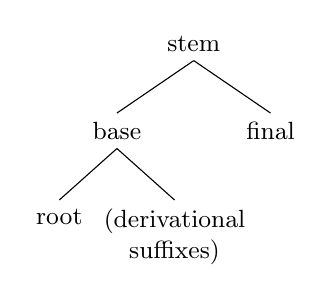
\begin{tikzpicture}[level distance=2.5em,
		sibling distance=8em,
		parent anchor=south,
		child anchor=north,
		anchor=north,
		align=center]
		\small
		\node{stem}
		child[sibling distance=6em]
		{node {base} edge from parent[solid]
			child[sibling distance=4.5em]
			{node {root} edge from parent[solid]}	
			child[sibling distance=4.5em]
			{node {(derivational\\suffixes)} edge from parent[solid]}
		}		
		child[sibling distance=6em]
		{node {final} edge from parent[solid]}
		
		;
		\end{tikzpicture}
		\captionabove{Hierarchical structure of the verb}\label{HierarchicalStructureVerb} 
	\end{center}
\end{figure} 

A number of verbs with initial /i/ are formally \isi{reflexive} verbs, that is, they are preceded by the reflexive object marker \textit{i}- (\sectref{Reflexive}). However, with some of these the reflexive semantics has become obscured and there may not exist a corresponding stem without the reflexive marker. There are at least two diagnostic criteria regarding the status of initial /i/. First, object prefixes do not count as stem syllables. Trisyllabic formal reflexives are thus treated as disyllabic in the formation of the perfective stem (see \sectref{Imbrication}).\is{imbrication}
\begin{exe}
	\ex
	\begin{tabbing}
		\textit{i-nogon-e!}x\=`turn (sthg.) upside down!'x\= > \textit{ikifiifye}x\=\kill
		\textit{itoga}\>`mount (horse, donkey)'\> > \textit{itogile}\>(not *\textit{itwige})\\
		\textit{ikifya}\>`do your best'\> > \textit{ikifiifye}\>(not *\textit{ikiifye})
	\end{tabbing}
\end{exe}

Second, any object prefix other than first person singular triggers a final vowel -\textit{e} in the imperative\is{mood!imperative} (\sectref{Imperative}) (\ref{exReflexiveFinalE}). Verbs in which initial /i/ is part of the stem have -\textit{a} (\ref{exInitialIStem}),
\begin{exe}
	\ex\label{exReflexiveFinalE}
	\begin{tabbing}
		\textit{i-nogon-e!}x\=`turn (sthg) upside down!'x\= > \textit{ikifiifye}x\=\kill
		\textit{i-jʊʊl-e!}\>`work hard!'\>(not *\textit{ijʊʊla})\\
		\textit{i-nogon-e!}\>`think!'\>(not *\textit{inogona})
	\end{tabbing} 
	\ex\label{exInitialIStem}
	\begin{tabbing}
		\textit{i-nogon-e!}x\=`turn (sthg) upside down!'x\=> \textit{ikifiifye}x\kill
		\textit{inamika!}\>`turn (sthg) upside down!'\\
		\textit{igʊla!}\>`open!'
	\end{tabbing}
\end{exe}

The final slot of the stem is obligatory and by default is occupied by the final vowel (\textsc{fv}) -\textit{a}, except for certain TMA paradigms and the defective verbs \textit{lɪ} and \textit{tɪ} (\sectref{DefectiveVerbsCopulae}). Following Bantuist tradition, throughout the rest of this study verbs are listed as stems, except when explicitly making reference to hierarchically lower structures. Note that the verb stem is generally not a possible morphological word in Nyakyusa.\footnote{The exception is the imperative (\sectref{Imperative}),\is{mood!imperative} for those verbs that can figure in this paradigm and are not monosyllabic.}
\is{root|)}\is{base|)}\is{stem|)}